\documentclass[12pt, t]{beamer}

%------------------------------------------------------------------------------
% configuration
%------------------------------------------------------------------------------
\RequirePackage{etex}
\usepackage{currfile-abspath}
\usepackage{../../themes/dbt}
\usepackage{catchfilebetweentags}

\setbeameroption{hide notes}
\setbeamertemplate{caption}{\raggedright\insertcaption\par}

\graphicspath{{images/}}
\getmainfile
\getabspath{\themainfile}
\let\mainabsdir\theabsdir
\let\mainabspath\theabspath

\newcommand{\insertcode}[2]{\lstinputlisting[label=samplecode, basicstyle=#1]{\mainabsdir/code/#2}}
\newcommand{\bi}{\begin{itemize}}
\newcommand{\ei}{\end{itemize}}
\newcommand{\ig}{\includegraphics}
\newcommand{\myhref}[1]{\href{#1}{\tt \scriptsize #1}}
\newcommand{\incnote}[1]{\note{\ExecuteMetaData[notes.tex]{#1}}}
\newcommand{\src}[2]{\vspace{-10pt}\caption{\href{#1}{\centering \tt \tiny [#2]}}}


%------------------------------------------------------------------------------
% title
%------------------------------------------------------------------------------
%------------------------------------------------------------------------------
% title
%------------------------------------------------------------------------------
% slide
\title{Systèmes d'exploitation pour l'embarqué}
\subtitle{UV 5.2 - Exécution et Concurrence}

\author{\href{}{Paul Blottière}}
\institute{
    \href{http://www.ensta-bretagne.fr/}{ENSTA Bretagne} \\[2pt]
    \href{}{\tt \scriptsize 2017 / 2018}
}
\date{
    \href{https://github.com/pblottiere}{\tt \scriptsize https://github.com/pblottiere} \\[2pt]
    %\href{blottiere.paul@gmail.com}{\tt \scriptsize blottiere.paul@gmail.com}
}

% info
\begin{document}

{
\setbeamertemplate{footline}{} % no page number here
\frame{
    \titlepage
} }

%------------------------------------------------------------------------------
% amélioration continue
%------------------------------------------------------------------------------
\begin{frame}{Amélioration continue}
    \subt{Contributions}
    \vspace{12pt}

    \begin{center}
    
\includegraphics[scale=0.7]{github.png}
    \end{center}

    \bi
    \itemsep12pt
    \item Dépôt du cours : \href{https://github.com/pblottiere/embsys}{\tt \scriptsize https://github.com/pblottiere/embsys}
    \item Souhaits d'amélioration, erreurs, idées de TP, ... : ouverture d'Issues (avec le bon label!)
    \item Apports de corrections : Pull Request
    \ei
\end{frame}




%<**lecture_content>
%------------------------------------------------------------------------------
% lecture
%------------------------------------------------------------------------------
\begin{frame}[plain,c]
    \centering
    \huge\textcolor{title}{Linux embarqué : compilation et outils}
\end{frame}

%------------------------------------------------------------------------------
% plan
%------------------------------------------------------------------------------
\begin{frame}{Plan}
    \subt{}
    \vspace{8pt}

    \begin{enumerate}
        \itemsep10pt
        \item Autotools et menuconfig
        \item Une distribution minimale
        \item Cross-compilation
        \item Compilation du kernel
        \item Busybox
        \item U-Boot
        \item Buildroot vs Yocto Project
        \item QEMU
        \item gdbserver
    \end{enumerate}

    \note {
    }
\end{frame}

%------------------------------------------------------------------------------
% rec1
%------------------------------------------------------------------------------
\begin{frame}{Autotools et menuconfig (1)}
    \subt{Les autotools}

    \vspace{15pt}
    Ensemble d'outils de build du projet GNU.

    \begin{figure}
        \centering
        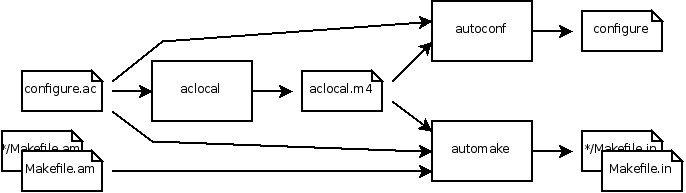
\includegraphics[scale=0.45]{autotools.png}
    \end{figure}

    \onslide<2->
    {
        \vspace{15pt}
        => très utilisé, aux côté de CMake!
    }
\end{frame}

%------------------------------------------------------------------------------
% rec2
%------------------------------------------------------------------------------
\defverbatim{\lstauto}
{
    \begin{lstlisting}
> ./configure
...
> make
...
> sudo make install
...
    \end{lstlisting}
}

\begin{frame}{Autotools et menuconfig (2)}
    \subt{Les autotools}

    \vspace{10pt}
    Utilisation classique sans paramétrage :
    \vspace{5pt}
    \lstauto

    \onslide<2->
    {
        \vspace{10pt}
        => par défaut, l'installation se fera avec le prefix {\textbf{/}} :
        \bi
        \itemsep8pt
        \item /usr/bin
        \item /usr/lib
        \item /usr/share
        \item ...
        \ei
    }
\end{frame}

%------------------------------------------------------------------------------
% rec3
%------------------------------------------------------------------------------
\begin{frame}{Autotools et menuconfig (3)}
    \subt{Les autotools}

    \vspace{10pt}
    La phase de configuration, via l'exécution de {\textit{./configure}},
    prend de nombreux paramètres en entrée :
    \vspace{5pt}
    \bi
    \itemsep8pt
    \item {\textit{- -build}} : système d'exécution courant
    \item {\textit{- -host}} : systèmes où le résultat de la compilation
          sera exécuté
    \item {\textit{- -prefix}} : prefix d'installation utilisé lors du
          {\textit{make install}}
    \item {\textit{- -enable-<FEATURE>}} : active la fonctionnalité
    \item {\textit{- -disable-FEATURE}} : désactive la fonctionnalité
    \item {\textit{- -help}} : affiche la liste des commandes disponibles
    \item ...
    \ei
\end{frame}

%------------------------------------------------------------------------------
% rec4
%------------------------------------------------------------------------------
\defverbatim{\lstconf}
{
    \begin{lstlisting}
> ./configure
checking build system type... x86_64-pc-linux-gnu
checking host system type... x86_64-pc-linux-gnu
...
checking for ncursesw/curses.h... no
checking ncurses.h usability... yes
checking ncurses.h presence... yes
checking for ncurses.h... yes
configure: creating ./config.status
config.status: creating Makefile
    \end{lstlisting}
}

\begin{frame}{Autotools et menuconfig (4)}
    \subt{Les autotools}

    \vspace{15pt}
    Un des rôles du script {\textit{configure}} est de vérifier la présence
    de toutes les dépendances et de construire les Makefile associés à partir
    des Makefile.in

    \onslide<2->
    {
        \vspace{15pt}
        \lstconf
    }
\end{frame}

%------------------------------------------------------------------------------
% rec5
%------------------------------------------------------------------------------
\begin{frame}{Autotools et menuconfig (5)}
    \subt{Menuconfig}

    \vspace{10pt}
    {\textbf{ncurses / New Curses}} : API de développement d'interface graphique
    simple en mode texte et exécutable dans un terminal.

    \onslide<2->
    {
        \vspace{10pt}
        {\textbf{kconfig}} : langage de configuration développé initialement par
        Linus Torvalds pour configurer le kernel à travers une IHM utilisant
        ncurses.
    }

    \onslide<3->
    {
        \vspace{10pt}
        => désormais, kconfig est utilisé par beaucoup d'autre projets de par sa
        légèreté et sa facilité d'utilisation :

        \bi
        \item kernel
        \item busybox
        \item crosstool-ng
        \item cross-builder
        \item ...
        \ei
    }
\end{frame}

%------------------------------------------------------------------------------
% rec6
%------------------------------------------------------------------------------
\defverbatim{\lstmenu}
{
    \begin{lstlisting}
> make menuconfig
    \end{lstlisting}
}

\begin{frame}{Autotools et menuconfig (6)}
    \subt{Menuconfig}

    \vspace{15pt}
    Par héritage, le lancement d'une IHM de configuration utilisant Kconfig se
    fait en exécutant la commande :

    \vspace{5pt}
    \lstmenu

    \onslide<2->
    {
        \begin{figure}
            \centering
            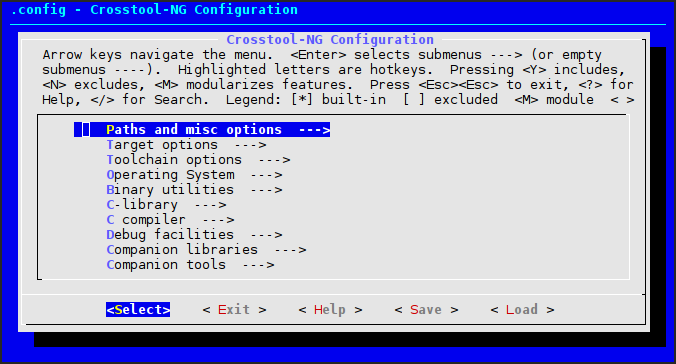
\includegraphics[scale=0.5]{ct-ng.png}
        \end{figure}
    }
\end{frame}

%------------------------------------------------------------------------------
% rec7
%------------------------------------------------------------------------------
\defverbatim{\lstkconf}
{
    \begin{lstlisting}
CONFIG_OID_REGISTRY=m
CONFIG_UCS2_STRING=y
CONFIG_FONT_SUPPORT=y
# CONFIG_FONTS is not set
CONFIG_FONT_8x8=y
CONFIG_FONT_8x16=y
CONFIG_ARCH_HAS_SG_CHAIN=y
CONFIG_ARCH_HAS_PMEM_API=y
    \end{lstlisting}
}

\begin{frame}{Autotools et menuconfig (7)}
    \subt{Menuconfig}

    \vspace{15pt}
    En sortie, un fichier de configuration, utilisé au moment du make, est
    généré à partir des éléments configurés dans l'interface :

    \vspace{10pt}
    \lstkconf

    \onslide<2->
    {
        => il existe souvent des fichiers de configuration prédéfinis pour des
        buts bien particuliers!
    }
\end{frame}

%------------------------------------------------------------------------------
% rec8
%------------------------------------------------------------------------------
\defverbatim{\lstkconf}
{
    \begin{lstlisting}
config MODVERSIONS
	bool "Set version info on module symbols"
	depends on MODULES
	help
        Usually, modules have to be recompiled
        whenever you switch to a new kernel.  ...
    \end{lstlisting}
}

\begin{frame}{Autotools et menuconfig (8)}
    \subt{Menuconfig}

    \vspace{15pt}
    Un exemple de script utilisant le langage KConfig :
    \vspace{5pt}
    \lstkconf
\end{frame}

%------------------------------------------------------------------------------
% mini1
%------------------------------------------------------------------------------
\begin{frame}{Une distribution minimale (1)}
    \subt{Kernel et RFS}

    \vspace{15pt}
    Une distribution minimale basée sur le noyau Linux nécessite seulement
    deux éléments :
    \bi
    \itemsep6pt
    \item un kernel
    \item un RFS contenant les binaires et les librairies de base
    \ei

    \begin{figure}
        \centering
        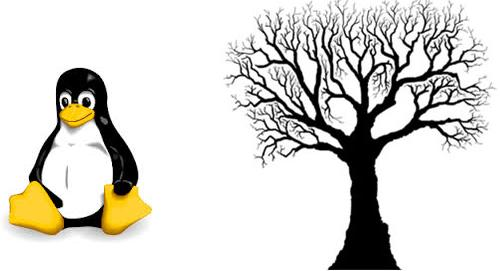
\includegraphics[scale=0.5]{kernel_root.jpeg}
    \end{figure}

\end{frame}

%------------------------------------------------------------------------------
% mini2
%------------------------------------------------------------------------------
\begin{frame}{Une distribution minimale (2)}
    \subt{Cross compiler}

    \vspace{15pt}
    Pour compiler l'ensemble, un élément est indispensable : {\textbf{un
    compilateur croisé}}.

    \onslide<2->
    {
        \begin{figure}
            \centering
            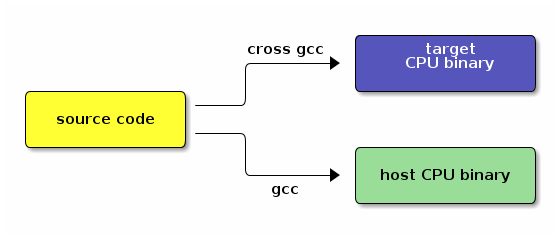
\includegraphics[scale=0.5]{cross_compile.png}
        \end{figure}
    }

    \onslide<3->
    {
        \vspace{5pt}
        => la première étape est donc de compiler le compilateur croisé.
    }
\end{frame}

%------------------------------------------------------------------------------
% cc1
%------------------------------------------------------------------------------
\begin{frame}{Compilateur croisé (1)}
    \subt{Contenu}

    \vspace{10pt}
    Une chaîne de compilation est difficile à mettre en oeuvre from scratch car
    elle contient de très nombreux éléments :

    \bi
    \itemsep6pt
    \item le compilateur en tant que tel : gcc-<ARCH>
    \item les outils fourni par GNU Binutils : ld, as, strip, nm, ...
    \item la libc : glibc, uclibc ou eglibc
    \ei

    \onslide<2->
    {
        \vspace{10pt}
        Il existe des chaînes sur étagère, robustes et éprouvées :
        \bi
        \itemsep6pt
        \item Crosstool (vieillisant)
        \item Crosstool-NG
        \item la chaîne de ELDK
        \item la chaîne de Buildroot
        \item la chaîne de Yocto Project
        \ei
    } 

\end{frame}

%------------------------------------------------------------------------------
% cc2
%------------------------------------------------------------------------------
\begin{frame}{Compilateur croisé (2)}
    \subt{Crosstool-NG}

    \vspace{10pt}
    Auteur : Yann Morin / Fançais / ENIB.

    \onslide<2->
    {
        \vspace{10pt}
        Les architectures supportées : ARM, AVR, PPC, x86, ...
    }

    \onslide<3->
    {
        \vspace{10pt}
        A travers la configuration de Crosstool-ng, on peut choisir
        l'architecture cible, la version de gcc, la libc, la version de la
        libc, ...
    }

    \onslide<4->
    {
        \begin{figure}
            \centering
            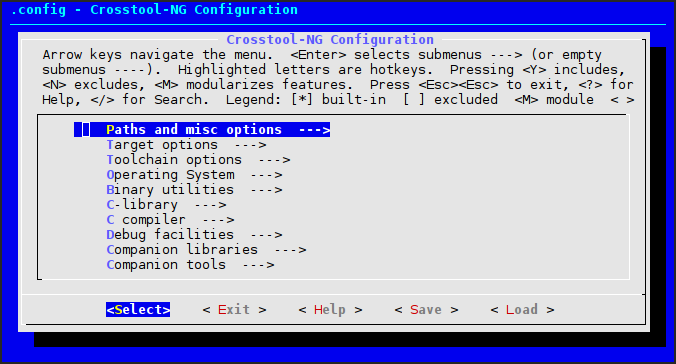
\includegraphics[scale=0.4]{ct-ng.png}
        \end{figure}
    }
\end{frame}

%------------------------------------------------------------------------------
% cc3
%------------------------------------------------------------------------------
\begin{frame}{Compilateur croisé (3)}
    \subt{ELDK}

    \vspace{15pt}
    Embedded Linux Development Kit :
    \bi
    \itemsep6pt
    \item chaîne de compilation croisée pour PPC, ARM ou MIPS
    \item distribution Linux associée à l'architecture cible
    \ei

    \onslide<2->
    {
        \vspace{15pt}
        => on peut très bien n'utiliser que la chaîne de compilation et
        construire nous même la distribution.
    }

    \onslide<3->
    {
        \vspace{15pt}
        => la chaîne de compilation de ELDK vient avec des librairies
        précompilées. On ne peut donc pas choisir les versions de gcc ou de la
        glibc
    }

    \onslide<4->
    {
        \vspace{-10pt}
        \begin{figure}
            \centering
            \hspace{140pt}
\includegraphics[scale=0.9]{denx.png}
        \end{figure}
    }
\end{frame}

%------------------------------------------------------------------------------
% cc4
%------------------------------------------------------------------------------
\begin{frame}{Compilateur croisé (4)}
    \subt{ISA et ABI}

    \vspace{5pt}
    {\textbf{Instruction Set Architecture}} : définie une interface de
    communication entre une brique logicielle et la partie matérielle.

    \onslide<2->
    {
        \vspace{5pt}
        {\textbf{Application Binary Interface}} : définie au niveau binaire une
        interface de communication entre plusieurs brique logiciel (librairies,
        OS, ...).
    }

    \onslide<3->
    {
        \begin{figure}
            \centering
            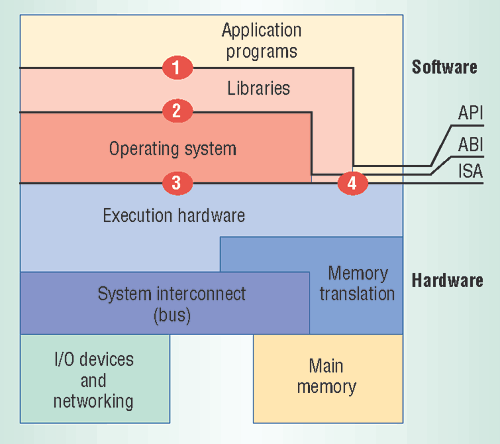
\includegraphics[scale=0.45]{abi-isa.png}
            \src{http://www.computer.org/csdl/mags/co/2005/05/r5032-abs.html}{ISA - ABI - API}
        \end{figure}
    }
\end{frame}

%------------------------------------------------------------------------------
% cc5
%------------------------------------------------------------------------------
\begin{frame}{Compilateur croisé (5)}
    \subt{ISA et ABI}

    \vspace{15pt}
    Il existe plusieurs ABI par architecture. On doit donc spécifier l'ABI
    souhaité au moment de la compilation de la chaîne de cross-compilation!

    \onslide<2->
    {
        \vspace{15pt}
        Le choix de l'ABI a une conséquence directe la taille du code généré,
        l'utilisation de la mémoire, ...
    }

    \onslide<3->
    {
        \vspace{15pt}
        Par exemple pour ARM :
        \bi
        \item OABI : Old-ABI
        \item EABI : Embedded-ABI
        \ei
    }
\end{frame}

%------------------------------------------------------------------------------
% cc6
%------------------------------------------------------------------------------
\begin{frame}{Compilateur croisé (6)}
    \subt{FPU}

    \vspace{15pt}
    {\textbf{Floating Point Unit}} : unité de calcul en virgule flottante.

    \vspace{15pt}
    => dans un processeur, il peut y avoir une partie dédiée aux opérations
    sur flottant.

    \onslide<2->
    {
        \vspace{15pt}
        Si un processeur ne possède pas de FPU (dit {\textit{hardware FPU}}),
        le calcul sur nombres flottant est exécuté logiciellement par le
        compilateur lors de la génération en langage machine.

        \vspace{15pt}
        => on parle alors non pas de {\textbf{hardfpu}}, mais de
        {\textbf{softfpu}}!
    }
\end{frame}

%------------------------------------------------------------------------------
% cc7
%------------------------------------------------------------------------------
\begin{frame}{Compilateur croisé (7)}
    \subt{OABI vs EABI : un problème de FPU}

    \vspace{15pt}
    OABI part du principe que le processeur possède une FPU. Or, toutes les
    cartes sous ARM n'en possède pas nécessairement.

    \onslide<2->
    {
        \vspace{15pt}
        Dans le cas d'une demande d'un calcul sur flottant avec une OABI mais
        sur un processeur n'ayant pas de FPU, une exception sera levée par le
        processeur, puis attrapée par le kernel qui va lui même utiliser sa
        fonction de {\textit{softfpu}}.
    }

    \onslide <3->
    {
        \vspace{15pt}
        => terriblement inefficace car même chose sur tous les calculs sur les
        flottants!
    }
\end{frame}

%------------------------------------------------------------------------------
% cc8
%------------------------------------------------------------------------------
\begin{frame}{Compilateur croisé (8)}
    \subt{OABI vs EABI : un problème de FPU}

    \vspace{15pt}
    EABI permet de gérer la fonction de {\textit{softfpu}} dans l'espace
    utilisateur au lieu de l'espace kernel, ce qui augmente les performances!

    \vspace{15pt}
    => pour cela, il faut passer des options à gcc au moment de la compilation!
\end{frame}

%------------------------------------------------------------------------------
% cc9
%------------------------------------------------------------------------------
\begin{frame}{Compilateur croisé (9)}
    \subt{OABI vs EABI : un problème de FPU}

    \begin{figure}
        \centering
        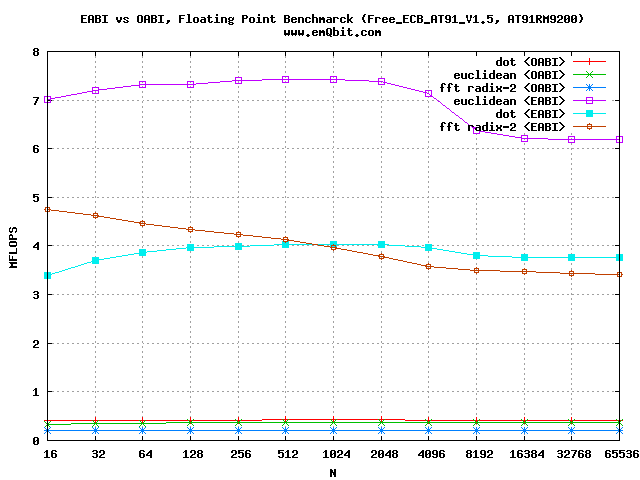
\includegraphics[scale=0.4]{benchmark.png}
        \src{http://archive.linuxgizmos.com/why-arms-eabi-matters/}{Benchmark OABI vs EABI}
    \end{figure}
\end{frame}

%------------------------------------------------------------------------------
% ker1
%------------------------------------------------------------------------------
\begin{frame}{Compilation du kernel (1)}
    \subt{Les sources}



\end{frame}

%------------------------------------------------------------------------------
% auto1
%------------------------------------------------------------------------------
\begin{frame}{Automatisation de la phase de build (1)}
    \subt{Buildroot}

    \vspace{15pt}
    Buildroot est un ensemble de Makefile automatisant le process de build
    d'une distribution Linux embarquée.

    \onslide<2->
    {
        \vspace{15pt}
        Pour la phase de cross-compilation, soit Buildroot en construit une, soit
        on lui indique d'utiliser une chaîne custom (comme celle de Crosstool-ng).
    }

    \onslide<3->
    {
        \vspace{15pt}
        Configurable à la {\textit{menuconfig}}.
    }

    \onslide<4->
    {
        \vspace{10pt}
        \begin{figure}
            \centering
            
\includegraphics[scale=0.35]{logo-buildroot.png}
        \end{figure}
    }
\end{frame}

%------------------------------------------------------------------------------
% auto2
%------------------------------------------------------------------------------
\begin{frame}{Automatisation de la phase de build (2)}
    \subt{Yocto Project}
\end{frame}

%------------------------------------------------------------------------------
% concl1
%------------------------------------------------------------------------------
\begin{frame}{Conclusion}

    \centering
    \vspace{20pt}
    \LARGE{
    }

\end{frame}

%------------------------------------------------------------------------------
% ref
%------------------------------------------------------------------------------
\begin{frame}{Références}
    \vspace{30pt}

    \bi
    \itemsep12pt
    \item https://github.com/torvalds/linux/tree/master/Documentation
    \item https://lwn.net/Kernel/LDD3/
    \item http://tldp.org/HOWTO/Serial-Programming-HOWTO/
    \item Linux Embarqué - Pierre Ficheux
    \ei

\end{frame}
%<//lecture_content>

\end{document}
